\section{Set Temperature}
\index{temperature}
Make sure to first read the instructions for using the Printrun software. Connect to the printer as described in the Printrun software section
%%% XXX pageref going to \label not \section
(page \pageref{Printrun}). Set the hot end and print surface for ABS plastic and turn both on. The temperature settings should be set at \texttt{230°C} for the hot end and \texttt{100°C} for print surface. If you have not already, make sure the axes end stops are aligned to be triggered when each axis homes. Click the \texttt{Motors Off} button.

\section{Load Filament}
\index{filament}
\index{hot end}
Once the hotend is heated to the correct temperature you will now need to load the plastic filament into the extruder. Loosen the two idler bolts (turn the black plastic knobs by hand) to take pressure off of the idler springs
(Fig. \ref{fig:extruder_idler_bolts}, page \pageref{fig:extruder_idler_bolts}).
\begin{figure}[hbt]
\centering
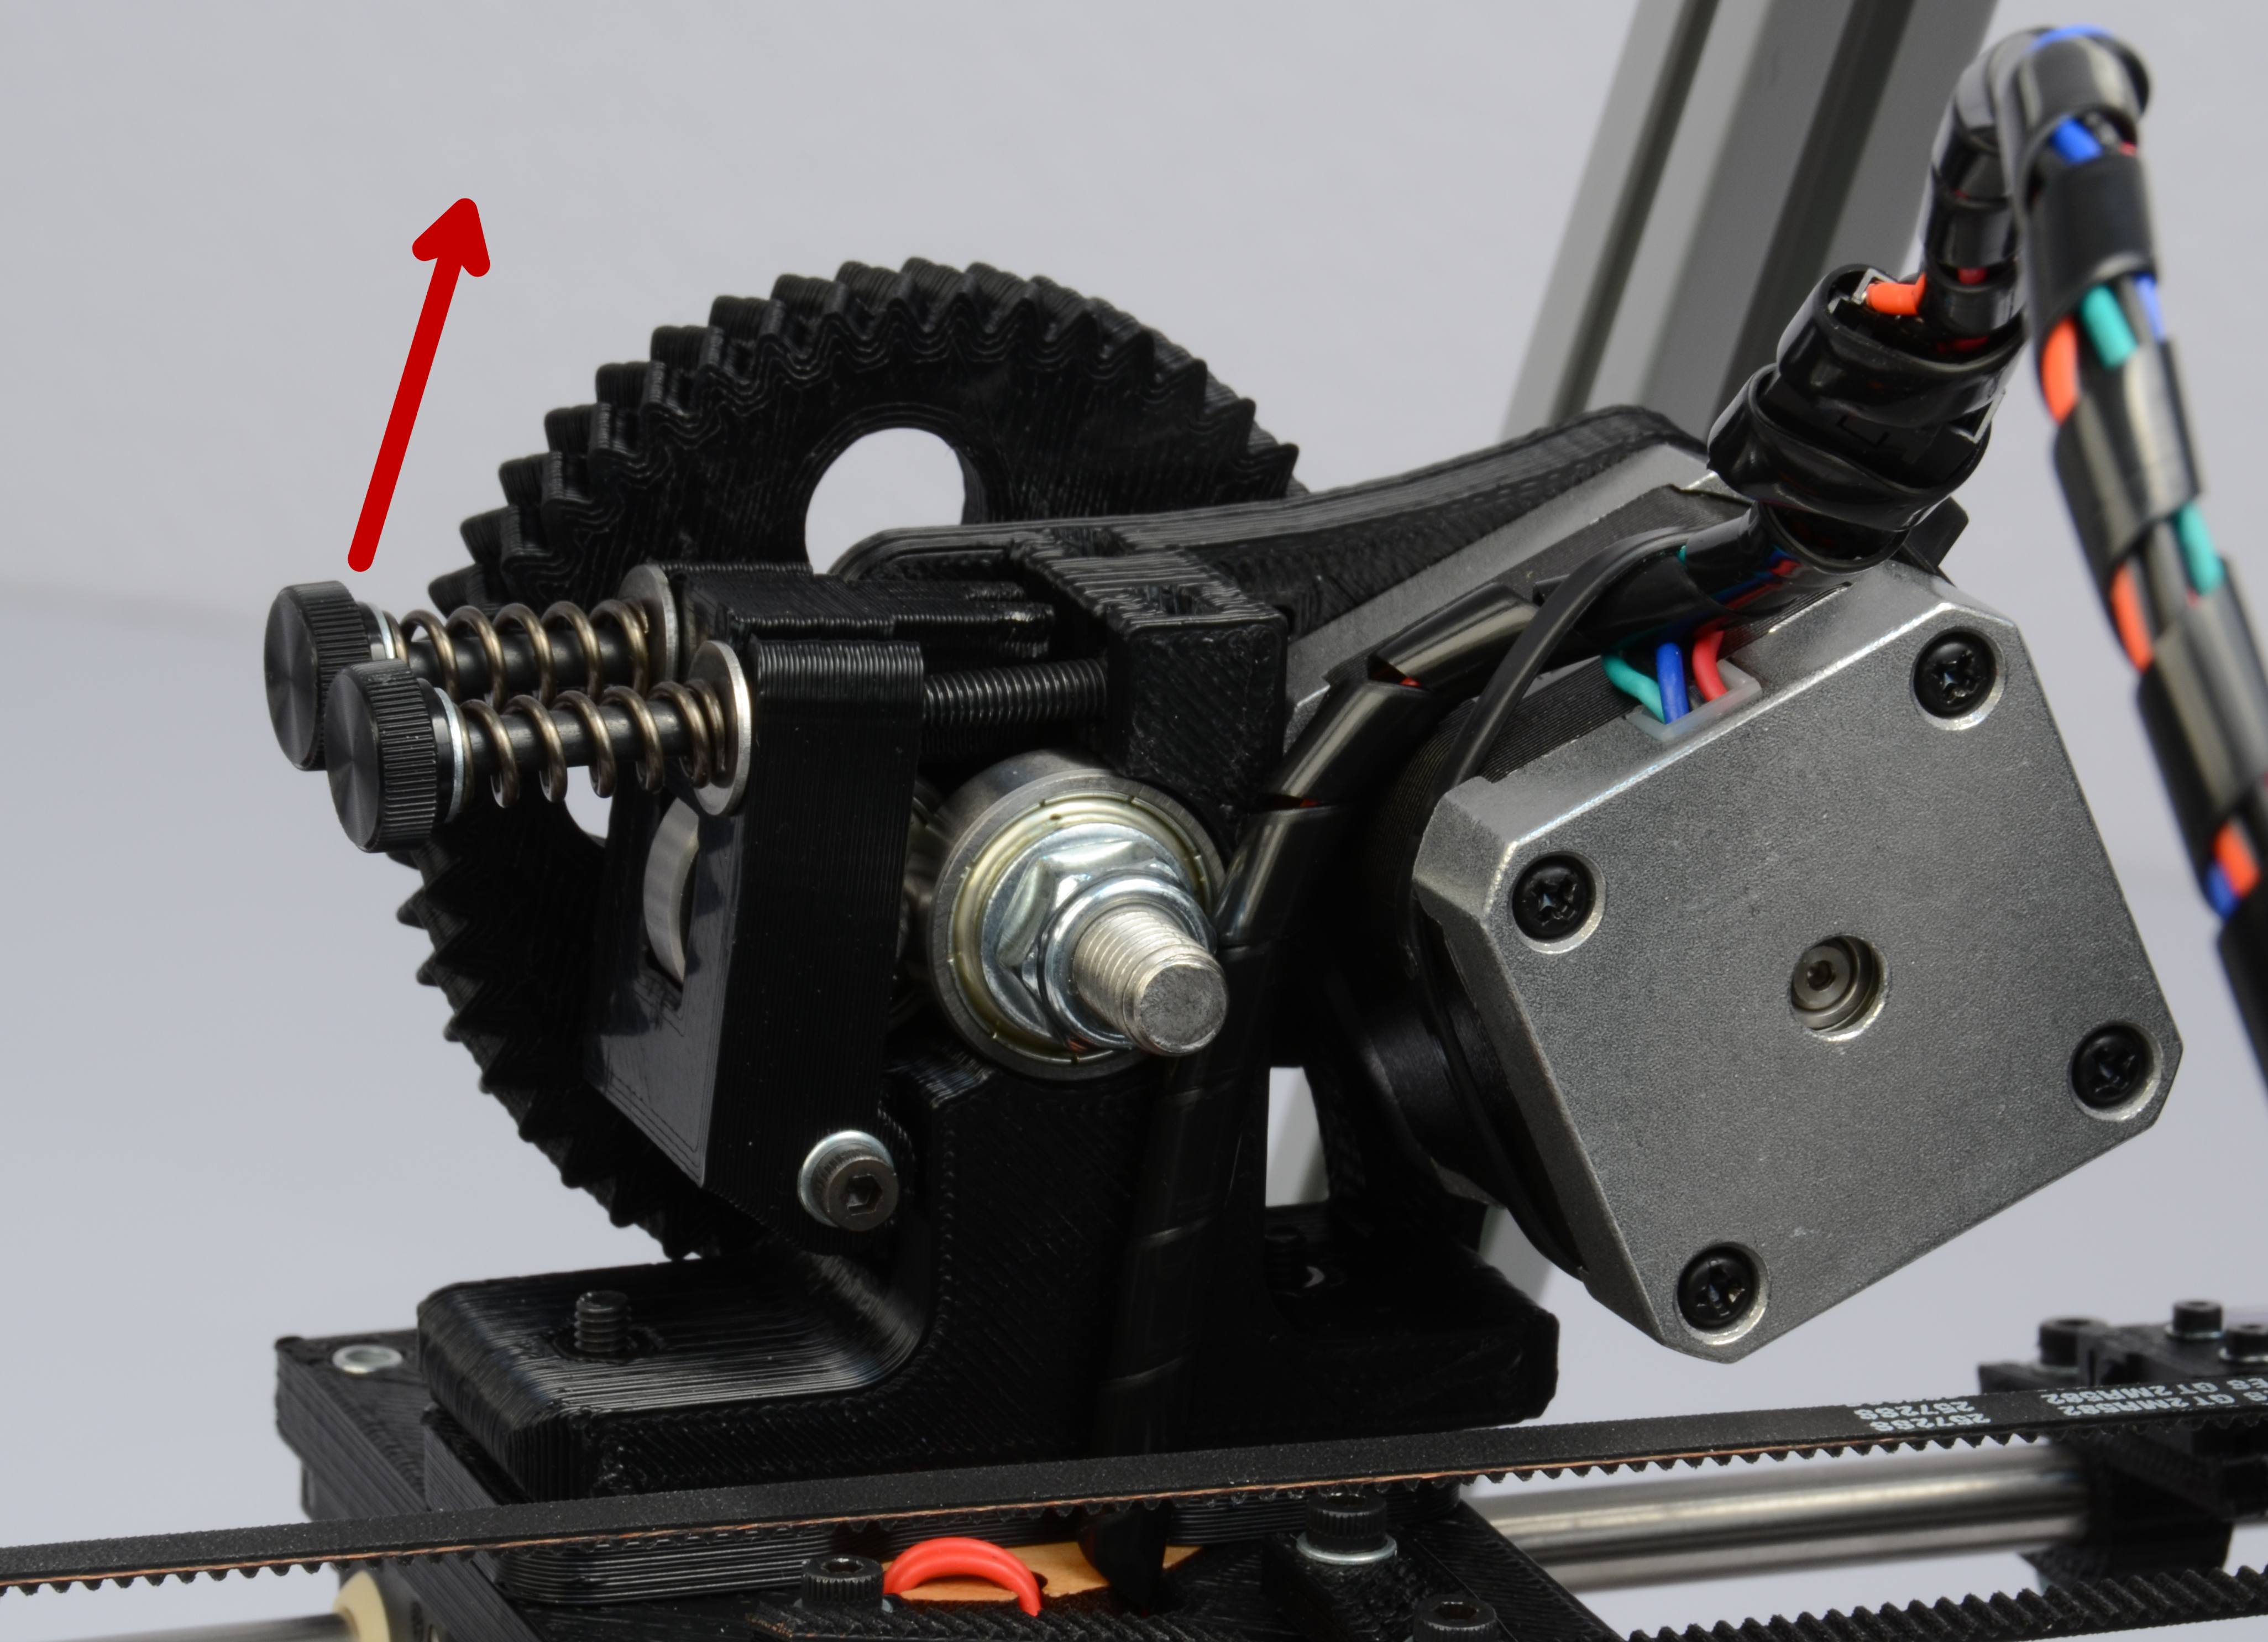
\includegraphics[keepaspectratio=true,angle=0,height=0.4\textheight,width=1.0\textwidth]{extruder_idler_bolts.jpg}
\caption{Extruder idler bolts}
\label{fig:extruder_idler_bolts}
\end{figure}
Pull both idler screws upwards to release the idler. The idler can be turned downwards allowing access to the hobbed bolt and filament feed hole. Feed the end of the plastic filament into the filament feed hole
(Fig. \ref{fig:extruder_feed_hole}, page \pageref{fig:extruder_feed_hole}).
\begin{figure}[hbt]
\centering
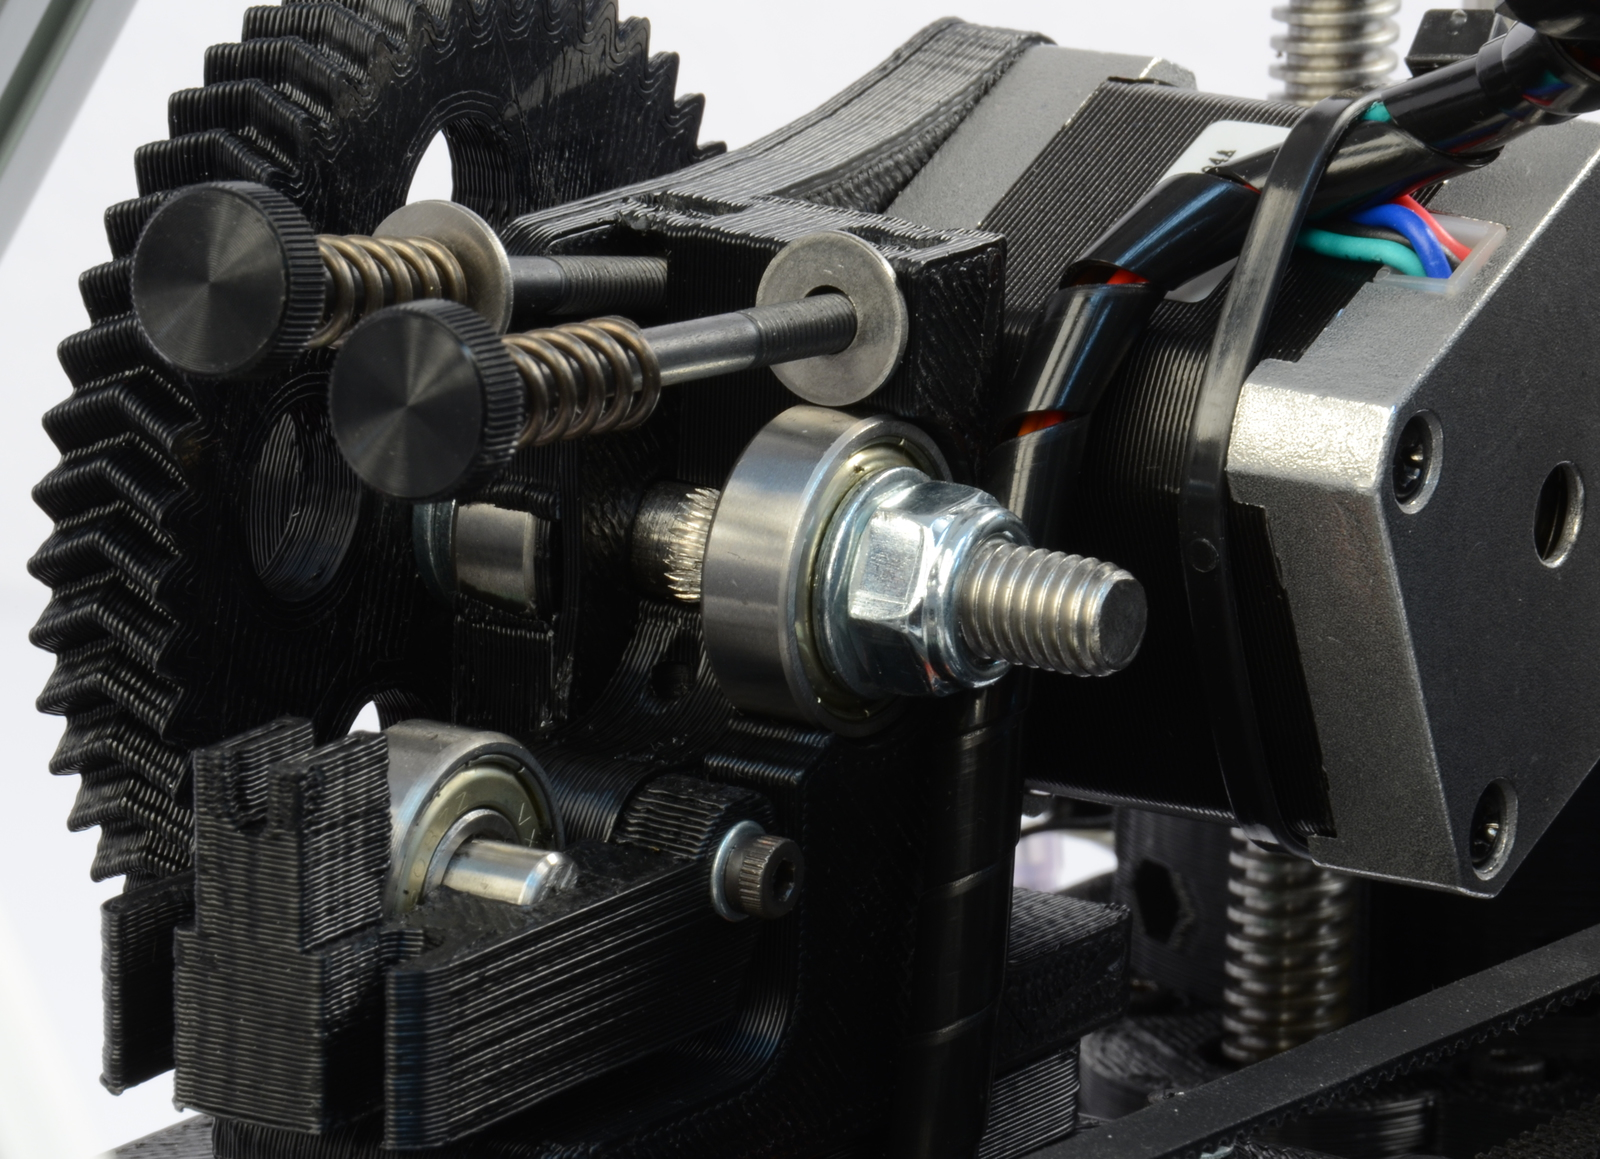
\includegraphics[keepaspectratio=true,angle=0,height=0.4\textheight,width=1.0\textwidth]{extruder_feed_hole.jpg}
\caption{Extruder feed hole}
\label{fig:extruder_feed_hole}
\end{figure}
Now you can push the filament through the extruder by slowly pushing the filament down into the hot end.

Once the filament extrudes a small amount out of the nozzle raise the idler and slide the two idler bolts and springs back into place. Tighten the two idler bolts so that the knobs are distanced 20mm away from the extruder body. Now use the \texttt{Extrude} button in Printrun to test that the extruder is working properly.

\section{Home Printer}
Use the home buttons to home the X axis and then the Y axis. Next home the Z axis. When the Z axis is at home the nozzle tip should be sitting right against the glass
(Fig. \ref{fig:nozzle_height}, page \pageref{fig:nozzle_height}). The image to the right, in figure \ref{fig:nozzle_height}, is the correct nozzle height.
\begin{figure}[hbt]
\centering
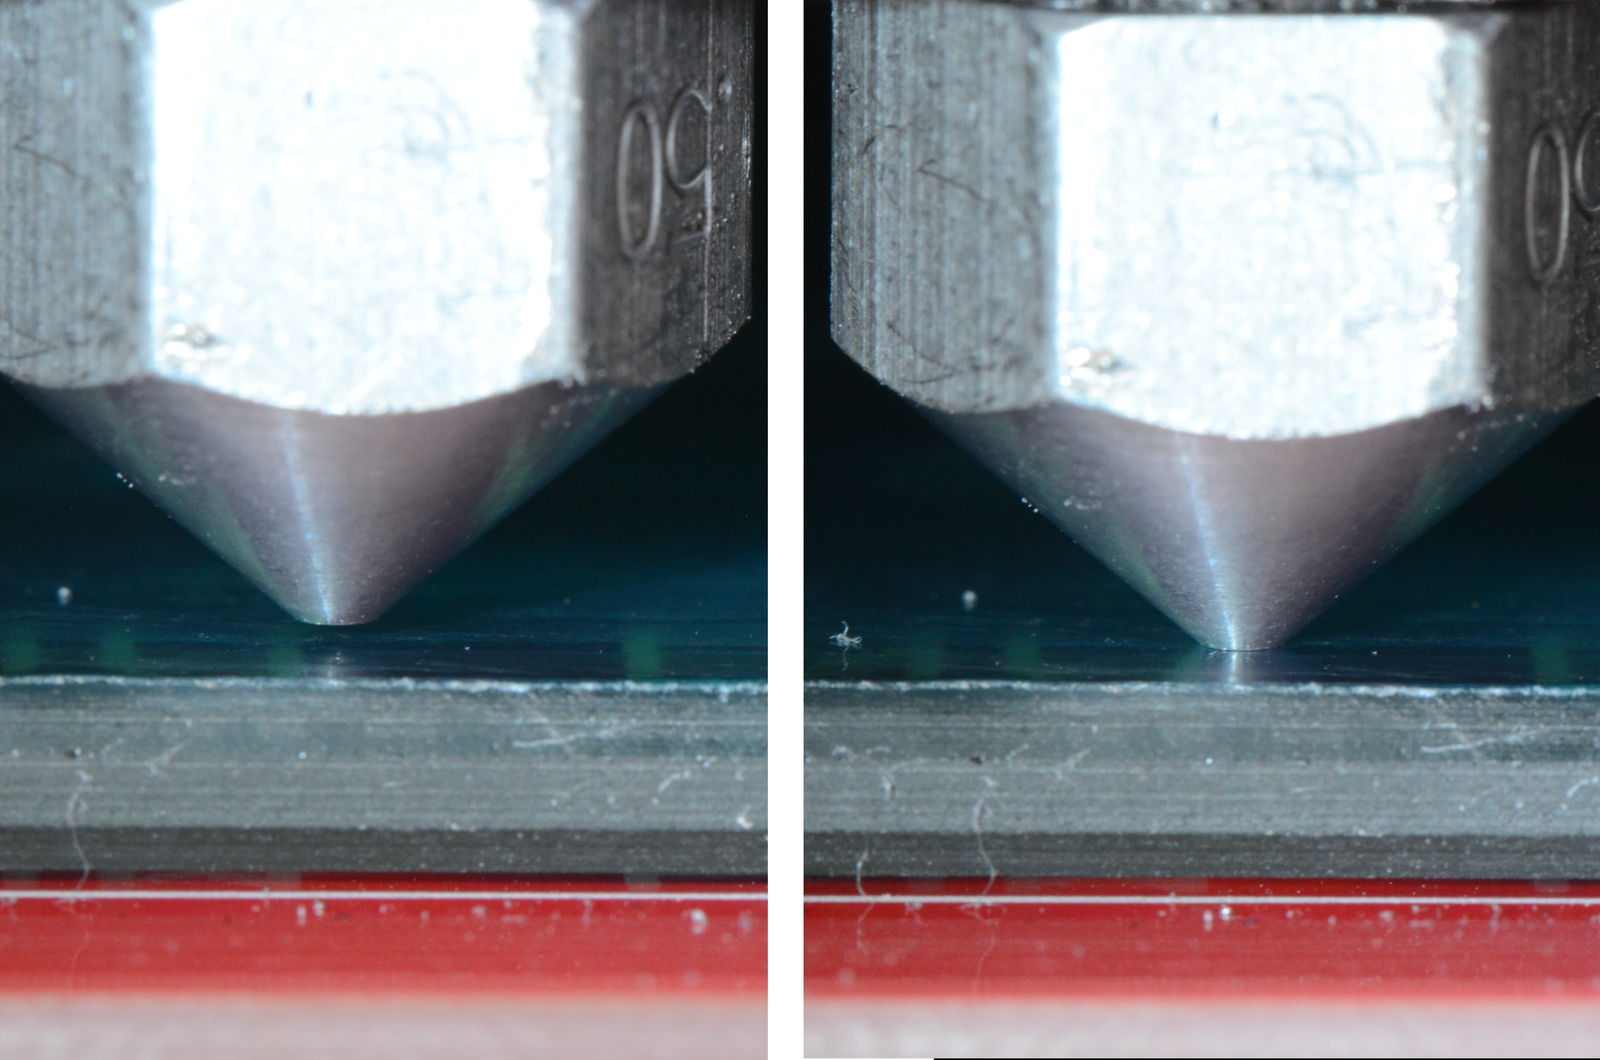
\includegraphics[keepaspectratio=true,angle=0,height=0.4\textheight,width=1.0\textwidth]{nozzle_height.jpg}
\caption{Nozzle height}
\label{fig:nozzle_height}
\end{figure}
The nozzle should not be pushing down on the print surface. To lower or raise the Z home height adjust the Z end stop trigger. The end stop trigger is on the far left of the printer near the print surface
(Fig. \ref{fig:z_endstop_trigger}, page \pageref{fig:z_endstop_trigger}).
\begin{figure}[hb!]
\centering
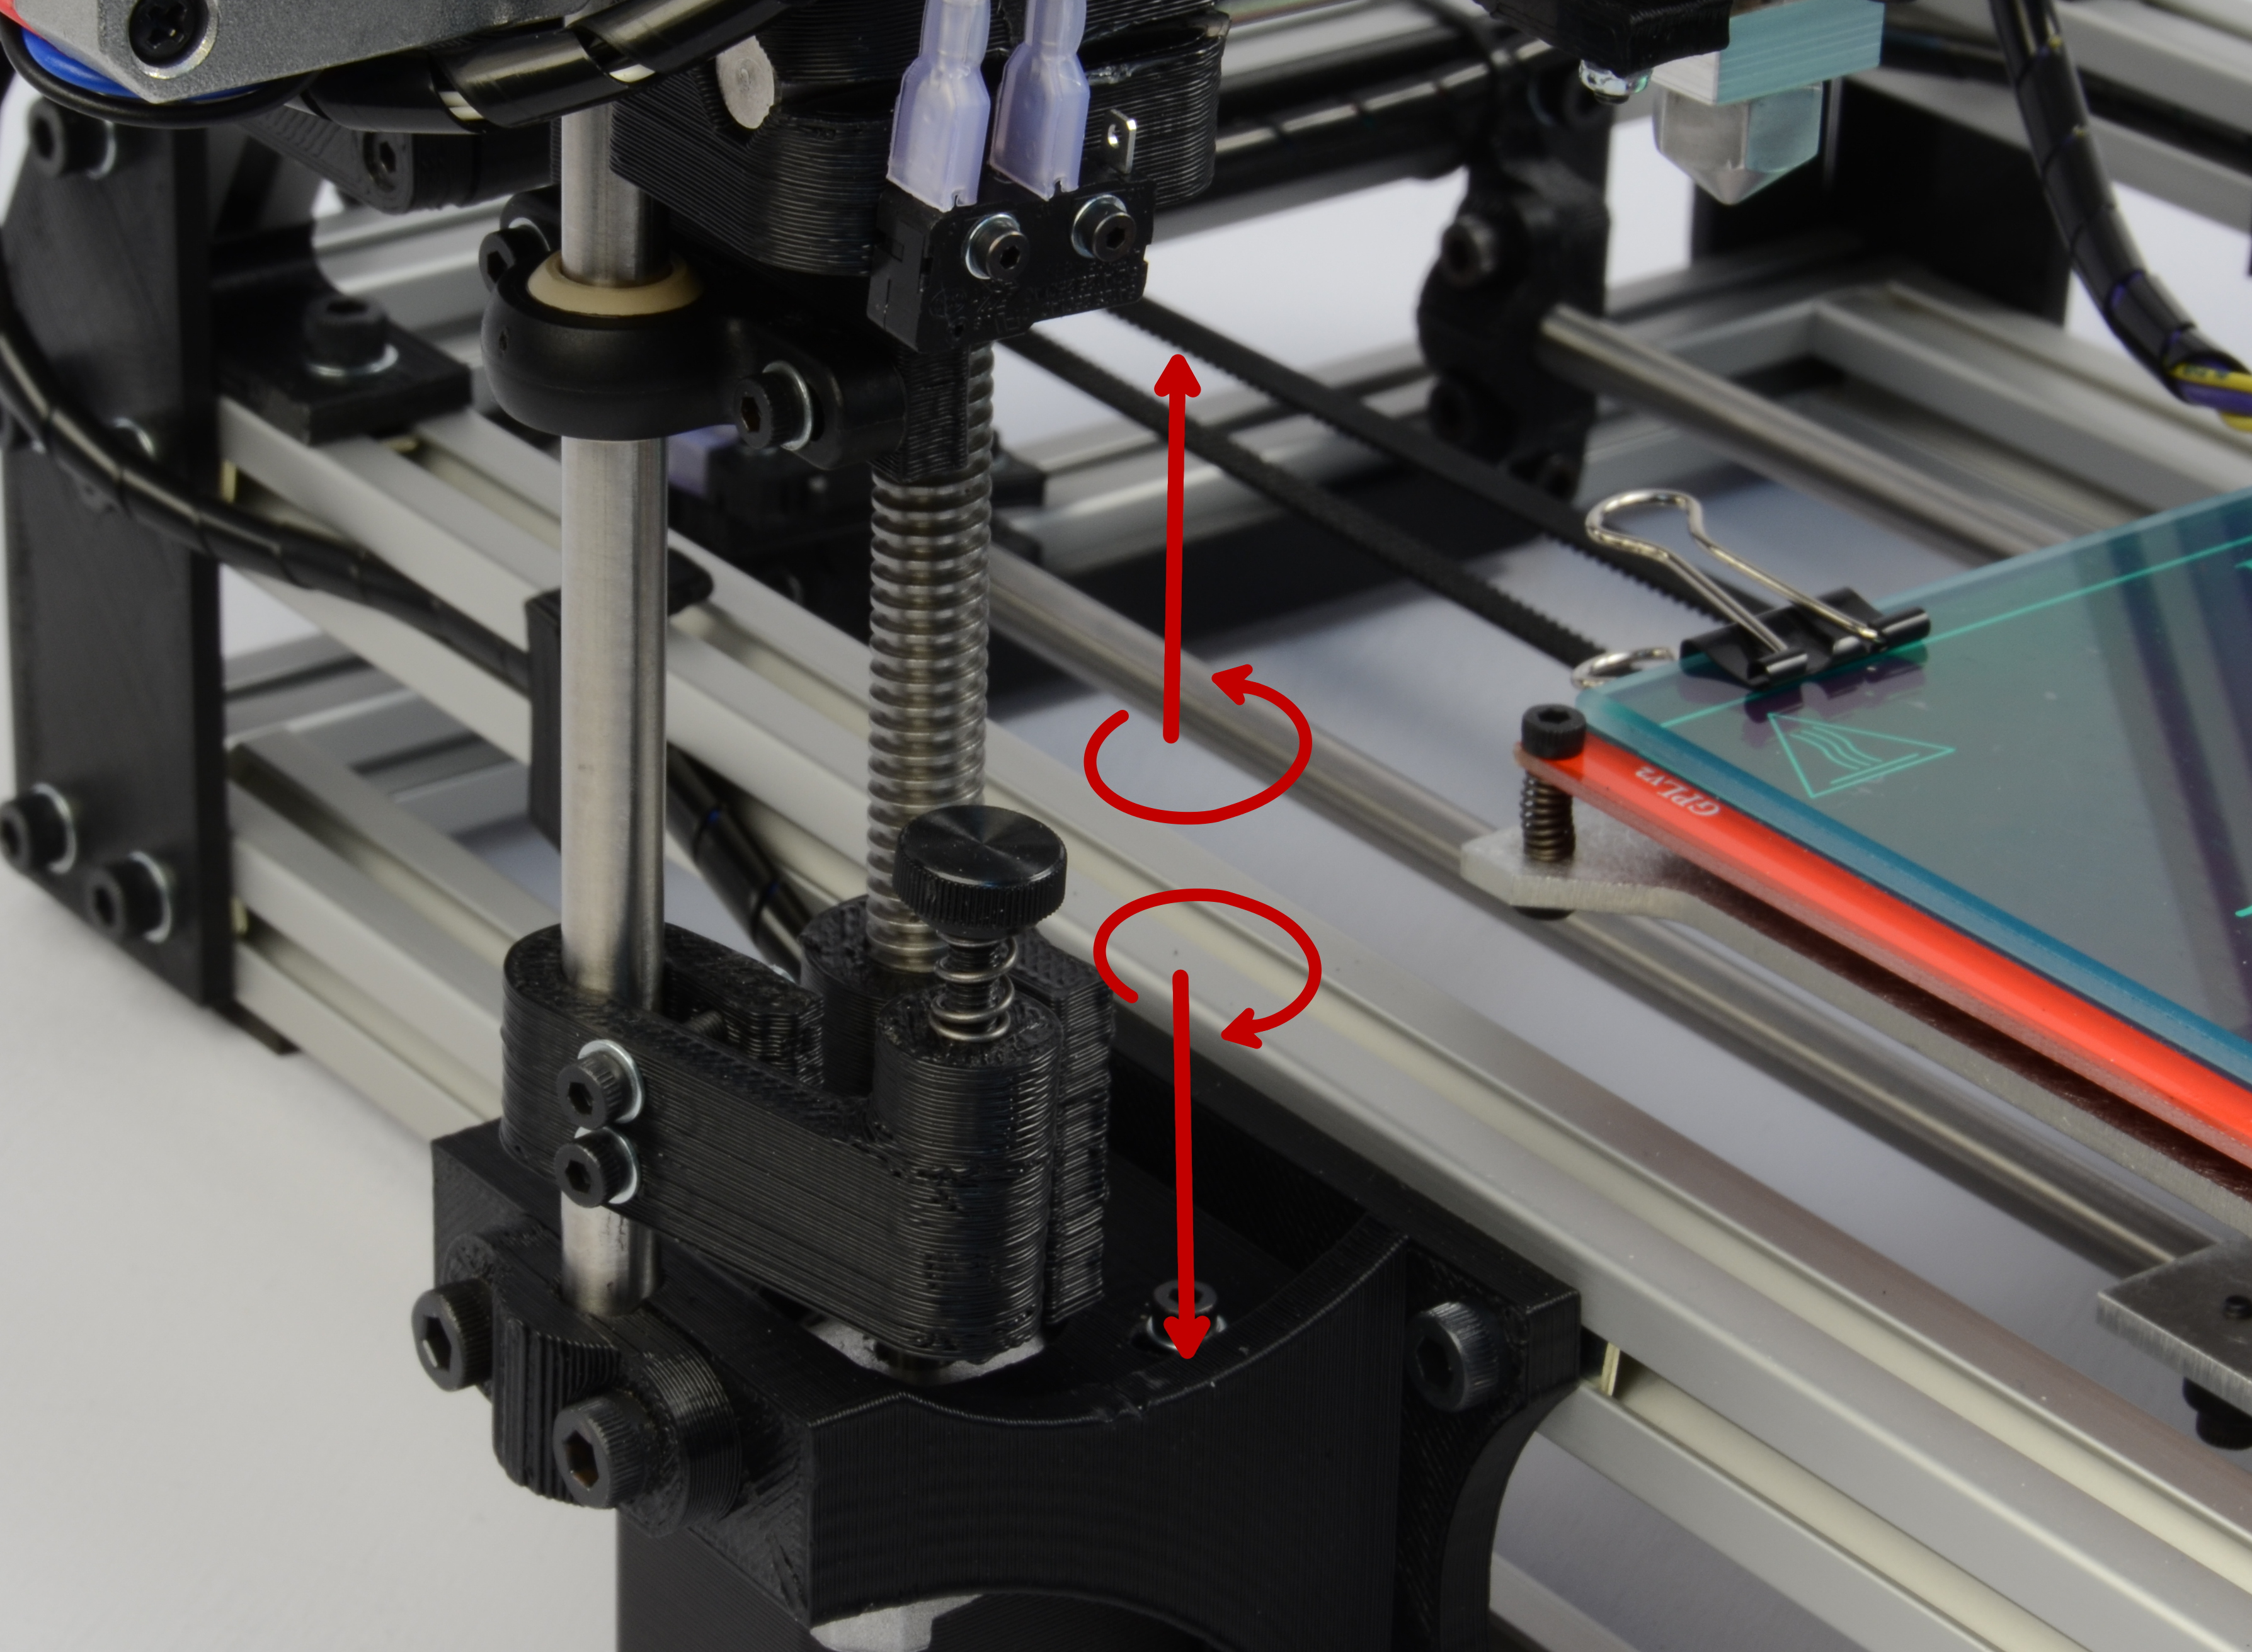
\includegraphics[keepaspectratio=true,angle=0,height=0.4\textheight,width=1.0\textwidth]{z_endstop_trigger.jpg}
\caption{Z endstop trigger}
\label{fig:z_endstop_trigger}
\end{figure}
The end stop trigger can be lowered by turning clockwise and raised by turning counter-clockwise. Once you have homed the axes and the hotend and bed have reached the correct temperature it is time to print!

\section{Z Print Height}
Load the \texttt{bedcalib.gco} file.
This file can be found at:
\texttt{http://download.lulzbot.com/TAZ/objects/calibration/bedcalib.gco}

The .gcode pattern should appear in the Printrun G-Code viewer. Press the \texttt{Print} button to begin the print. When the print starts make sure the first layer is not printing too close or too far from the print bed. Note 
Figure \ref{fig:1st_layer_adhesion}, page \pageref{fig:1st_layer_adhesion},
\begin{figure}[hbt]
\centering
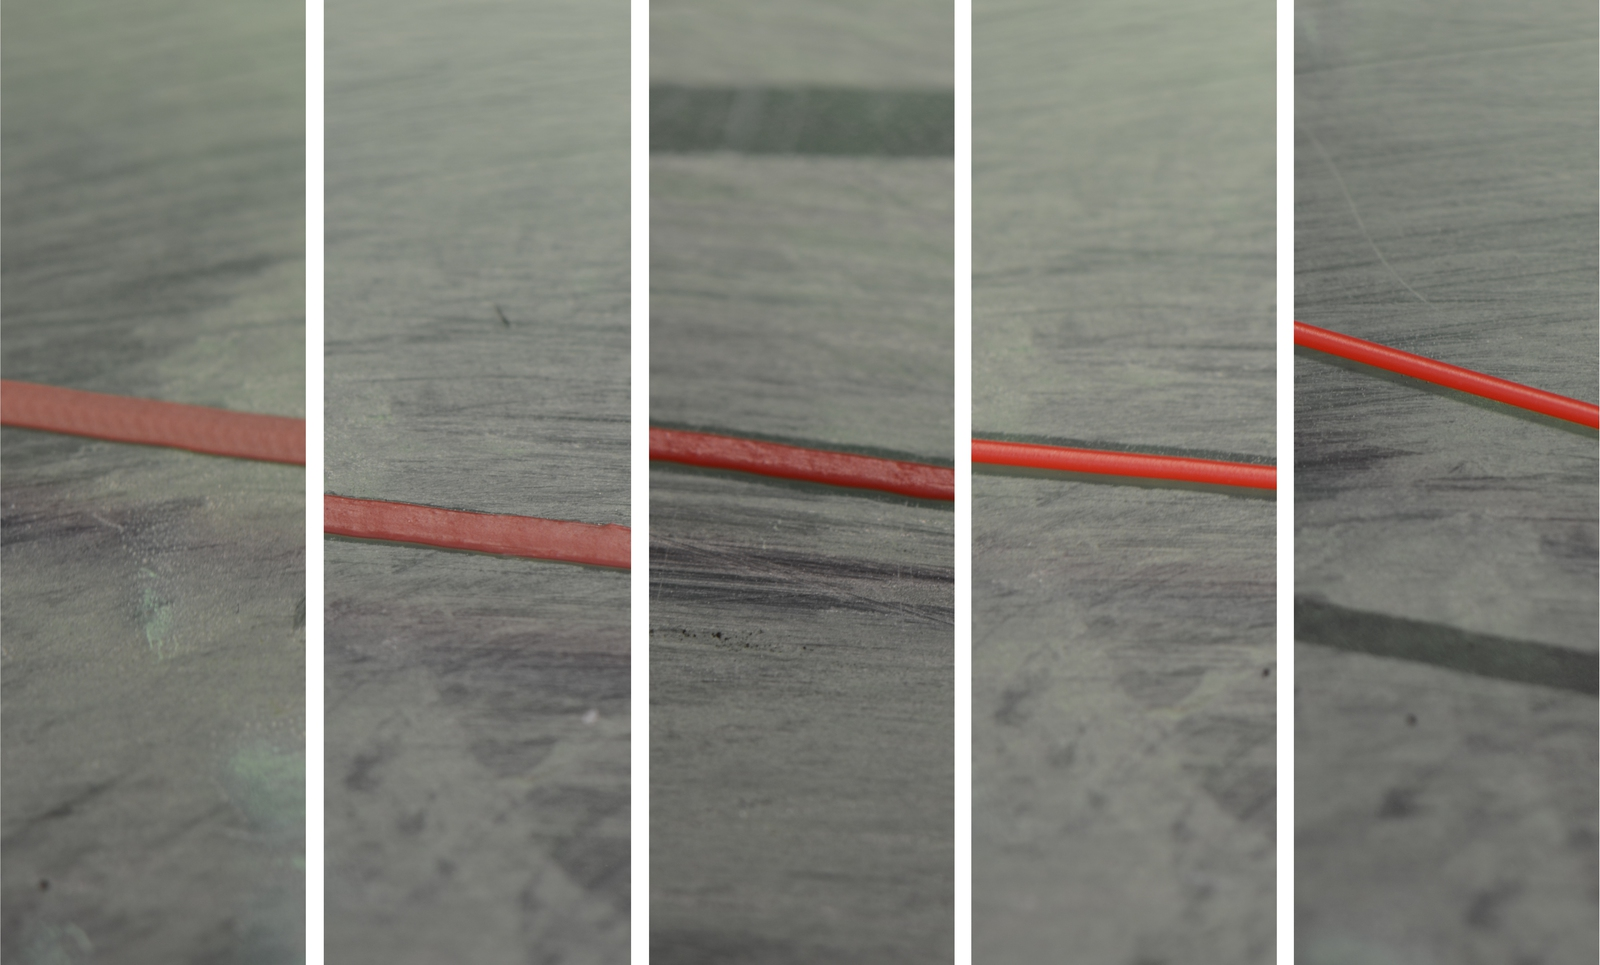
\includegraphics[keepaspectratio=true,angle=0,height=0.4\textheight,width=1.0\textwidth]{1st_layer_adhesion.jpg}
\caption{First layer adhesion}
\label{fig:1st_layer_adhesion}
\end{figure}
as an example of a good first layer adhesion. From left to right: very low, low, \emph{perfect,} high, very high. If the first layer is too high or low you can pause the print by pressing the \texttt{Pause} button. Adjust the Z end stop trigger. After making adjustments you can home the axes and press \texttt{Restart} to restart the print.

\section{Remove Part}
After the part is finished printing, the heated bed will automatically cool down to \texttt{60°C}. If you are printing PLA you will need to turn the heated bed off. Once the bed cools you can you pop the finished part off of the printed surface. To remove the printed part, use the clam knife included in your printer kit. Leather gloves are suggested to protect your hands from the clam knife blade. It is also safe practice to not place your hand behind the direction you are pushing the clam knife. Using the side of the clam knife blade pry up one side of the printed part. If your part is large you may need to pry at multiple points to pop the part off of the print surface. When removing parts take caution to not damage the PET film. If the film is cut or ripped it will peel from the glass and need to be replaced. Make sure to reset the heated bed to the correct temperature and allow it to heat up to the needed temperature before starting the next print.

